\documentclass[12pt]{article}

% Idioma e codificação
\usepackage[brazil]{babel}
\usepackage[utf8]{inputenc}
\usepackage[T1]{fontenc}

% Matemática e listas
\usepackage{amsmath, amssymb}
\usepackage{enumitem}
\usepackage{graphicx}
\usepackage{float} % <-- necessário para [H]

% Layout e cores
\usepackage{geometry}
\usepackage{graphicx}
\usepackage{xcolor}

% Cores institucionais
\definecolor{maincolor}{RGB}{0,100,50}
\definecolor{forestgreen}{RGB}{0,100,50}

% Cabeçalho e rodapé
\usepackage{fancyhdr}

% Blocos
\usepackage[most]{tcolorbox}
\newtcolorbox{block}[1]{%
  colback=green!5,
  colframe=maincolor,
  coltitle=white,
  title=#1,
  fonttitle=\bfseries,
  boxrule=1.5pt,
  arc=3mm,
  left=6pt,
  right=6pt,
  top=6pt,
  bottom=6pt
}

% Margens
\geometry{margin=2.5cm}

% Fancyhdr
\pagestyle{fancy}
\fancyhf{}

\renewcommand{\headrulewidth}{2pt}
\renewcommand{\footrulewidth}{2pt}

\renewcommand{\headrule}{\hbox to\headwidth{%
  \color{forestgreen}\leaders\hrule height \headrulewidth\hfill}}

\renewcommand{\footrule}{\hbox to\headwidth{%
  \color{forestgreen}\leaders\hrule height \footrulewidth\hfill}}

% Altura do cabeçalho (corrigida)
\setlength{\headheight}{52pt}
\addtolength{\topmargin}{-20pt}

% Cabeçalho
\fancyhead[L]{%
  
\includegraphics[height=1.2cm]{Universidade_de_Rio_Verde.jpg}
}

\fancyhead[R]{%
  \raggedleft
  \textcolor{forestgreen}{%
    \small
    \textbf{Lista de Exercícios}\\
    Me.~Sergio Souza Novak\\
    \textit{Banco de Dados}
    }
    }
    
    % Rodapé
    \fancyfoot[C]{\textcolor{forestgreen}{\thepage}}
    
    % =========================
    \begin{document}
    % =========================
    
    \vspace*{0.2cm}

    

\begin{center}
    \Large \textbf{Atividade Prática — Modelagem Entidade-Relacionamento} \\
    \normalsize Disciplina: Banco de Dados \\
    \normalsize Tema: Sistema de Ordenha de Vacas Leiteiras
\end{center}

\vspace{0.5cm}

\section*{Objetivo}
O objetivo desta atividade é desenvolver a capacidade de análise de requisitos e
modelagem conceitual de um banco de dados por meio da construção de um
\textbf{Diagrama Entidade-Relacionamento (DER)} para um sistema realista de
controle de ordenha em uma fazenda leiteira.

\section*{Contexto do Sistema}

\begin{figure}[H]
    \centering
    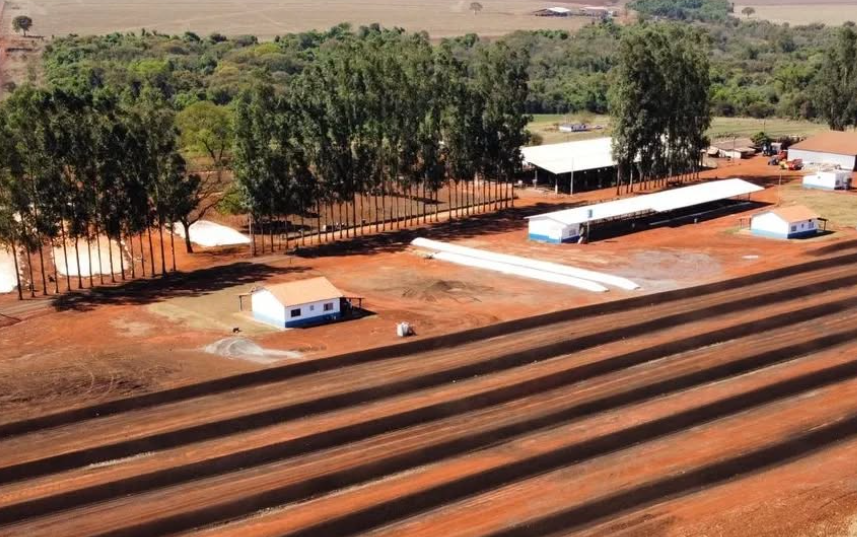
\includegraphics[width=9cm]{fazenda.png}
    \caption{Uma fazenda da cidade de Rio Verde. Fonte: Instagram @fazendanycolle}
\end{figure}

Uma fazenda leiteira deseja informatizar o controle de suas atividades de ordenha.
Atualmente, os registros são feitos manualmente, o que dificulta o acompanhamento
da produção, da saúde dos animais e do desempenho dos funcionários. O sistema deverá armazenar informações sobre as vacas, as ordenhas realizadas,
os funcionários responsáveis, os equipamentos utilizados e a produção de leite
obtida em cada ordenha.

\section*{Descrição dos Requisitos}

\subsection*{Vacas}
Cada vaca da fazenda deve ser identificada por um código único.
Além disso, devem ser armazenadas informações como:
\begin{itemize}
    \item Nome ou identificação visual;
    \item Data de nascimento;
    \item Raça;
    \item Peso;
    \item Status de saúde (por exemplo: saudável, em tratamento, isolada).
\end{itemize}

\subsection*{Funcionários}
A fazenda possui funcionários responsáveis pela ordenha.
Para cada funcionário, devem ser registrados:
\begin{itemize}
    \item Código de identificação;
    \item Nome completo;
    \item Função (ordenhador, veterinário, supervisor, etc.);
    \item Telefone.
\end{itemize}

\subsection*{Ordenha}
A ordenha ocorre diariamente e pode acontecer mais de uma vez por dia para a mesma vaca.
Cada ordenha deve registrar:
\begin{itemize}
    \item Data;
    \item Horário;
    \item Quantidade de leite produzida (em litros);
\end{itemize}

Uma ordenha:
\begin{itemize}
    \item Está associada a exatamente uma vaca;
    \item É realizada por um funcionário;
    \item Pode utilizar um ou mais equipamentos de ordenha.
\end{itemize}

\subsection*{Equipamentos}
A fazenda possui diversos equipamentos de ordenha.
Para cada equipamento, devem ser armazenadas as seguintes informações:
\begin{itemize}
    \item Código do equipamento;
    \item Tipo (manual, automático, robótico, etc.);
    \item Data da última manutenção;
    \item Situação (em uso, em manutenção, indisponível).
\end{itemize}

\subsection*{Supervisor}
Além dos funcionários da ordenha, a fazenda conta com um supervisor responsável
por acompanhar o trabalho diário.

Para cada supervisor, devem ser registradas informações como:
\begin{itemize}
    \item Código de identificação;
    \item Nome completo;
    \item Telefone de contato;
    \item Turno ou período de supervisão.
\end{itemize}

O supervisor acompanha as ordenhas realizadas e verifica se os procedimentos
estão sendo seguidos corretamente.
\subsection*{Veterinário}
A fazenda possui veterinários responsáveis pela saúde das vacas.
Eles realizam avaliações, tratamentos e acompanham o estado de saúde dos animais.

Para cada veterinário, devem ser armazenadas informações como:
\begin{itemize}
    \item Código de identificação;
    \item Nome completo;
    \item Registro profissional;
    \item Telefone de contato.
\end{itemize}

O veterinário pode atender várias vacas ao longo do tempo, e uma vaca pode
receber atendimento veterinário em diferentes momentos.
\subsection*{Proprietário}
O proprietário é o responsável geral pela fazenda.
Ele acompanha os relatórios de produção e toma decisões administrativas
com base nos dados registrados no sistema.

Para o proprietário, devem ser armazenadas informações como:
\begin{itemize}
    \item Código de identificação;
    \item Nome completo;
    \item Telefone de contato.
\end{itemize}

\begin{block}{Rotina de Ordenha}
Cada vaca da fazenda é ordenhada ao longo do tempo, normalmente todos os dias.
Em alguns períodos, a mesma vaca pode ser ordenhada mais de uma vez no mesmo dia.
Sempre que ocorre uma ordenha, ela diz respeito a uma única vaca.
\end{block}

\begin{block}{Trabalho dos Funcionários}
Os funcionários são responsáveis por realizar as ordenhas.
Um mesmo funcionário pode ordenhar várias vacas ao longo do dia.
No entanto, toda ordenha precisa ter alguém responsável por realizá-la.
\end{block}

\begin{block}{Uso dos Equipamentos}
Para realizar a ordenha, são utilizados equipamentos apropriados.
Dependendo da situação, podem ser usados um ou vários equipamentos em uma mesma ordenha.
Os equipamentos da fazenda podem ser utilizados em diferentes ordenhas ou
ficar temporariamente sem uso, quando estão em manutenção ou indisponíveis.
\end{block}
\begin{block}{Acompanhamento do Supervisor}
Durante o dia, o supervisor passa pelas áreas de ordenha para conferir se
o serviço está sendo feito corretamente.
Ele acompanha várias ordenhas e diferentes funcionários, mas nem sempre
precisa estar presente em todas elas.
\end{block}
\begin{block}{Cuidado com a Saúde das Vacas}
Quando alguma vaca apresenta problema de saúde, eu chamo o veterinário.
Ele pode atender várias vacas ao longo do tempo e, dependendo do caso,
a mesma vaca pode precisar de mais de um atendimento.
Esses cuidados ajudam a manter a produção e o bem-estar do animal.
\end{block}
\begin{block}{Visão do Proprietário}
Como proprietário, eu não participo da ordenha diretamente.
Meu interesse é acompanhar os resultados: quanto cada vaca produz,
como está o trabalho da equipe e se os equipamentos estão sendo bem utilizados.
Uso essas informações para tomar decisões sobre a fazenda.
\end{block}

\begin{block}{Registro da Produção}
A cada ordenha realizada, o produtor registra a data, o horário e a quantidade
de leite obtida.
Essas informações permitem acompanhar a produção de cada vaca e o desempenho
dos funcionários ao longo do tempo.
\end{block}
\section*{Atividades Propostas}

\begin{enumerate}[label=\alph*)]
    \item Identifique todas as \textbf{entidades} do sistema descrito.
    \item Para cada entidade, defina seus \textbf{atributos}, indicando a \textbf{chave primária}.
    \item Identifique e modele todos os \textbf{relacionamentos} existentes entre as entidades.
    \item Defina corretamente as \textbf{cardinalidades} (1:1, 1:N, N:M) e as \textbf{participações}
    (total ou parcial).
    


    \item Indique, quando necessário, atributos dos relacionamentos.
\end{enumerate}
\section*{Como as Informações do Sistema se Relacionam}

Para facilitar o entendimento do funcionamento da fazenda, o produtor descreve
o dia a dia da ordenha da seguinte forma:



\section*{Entrega}
\begin{itemize}
    \item O Diagrama Entidade-Relacionamento deve ser feito à mão (legível) ou utilizando
    uma ferramenta de modelagem (brModelo, Draw.io, Lucidchart, etc.).
    \item A entrega deve conter apenas o DER.
    \item Formato de entrega: PDF.
\end{itemize}

\section*{Critérios de Avaliação}
\begin{itemize}
    \item Correta identificação das entidades;
    \item Adequação dos atributos e chaves;
    \item Correção das cardinalidades e participações;
    \item Clareza e organização do diagrama;
    \item Coerência com o problema proposto.
\end{itemize}

\vspace{0.5cm}
\begin{center}
    \textbf{Boa atividade!}
\end{center}

 
% =========================
\end{document}
% =========================
